\documentclass[12pt,a4paper]{report}

% ============================================================================
% PACKAGES
% ============================================================================
\usepackage[utf8]{inputenc}
\usepackage[T1]{fontenc}
\usepackage{lmodern}
\usepackage[left=1.5in,right=1in,top=1in,bottom=1in]{geometry}
\usepackage{graphicx}
\usepackage{float}
\usepackage{amsmath}
\usepackage{amssymb}
\usepackage{xcolor}
\usepackage{colortbl}
\usepackage{hyperref}
\usepackage{tikz}
\usepackage{pgfplots}
\pgfplotsset{compat=1.18}
\usepackage{booktabs}
\usepackage{multirow}
\usepackage{enumitem}
\usepackage{fancyhdr}
\usepackage{tocloft}
\usepackage{titlesec}
\usepackage{caption}
\usepackage{subcaption}

% ============================================================================
% HYPERLINKS CONFIGURATION
% ============================================================================
\hypersetup{
    colorlinks=true,
    linkcolor=blue,
    filecolor=magenta,      
    urlcolor=cyan,
    citecolor=green,
}

% ============================================================================
% HEADER/FOOTER SETUP
% ============================================================================
\pagestyle{fancy}
\fancyhf{}
\fancyhead[L]{\leftmark}
\fancyhead[R]{\thepage}
\renewcommand{\headrulewidth}{0.5pt}

% ============================================================================
% TITLE PAGE
% ============================================================================
\begin{document}

\begin{titlepage}
    \centering
    \vspace*{3cm}
    
    {\Huge\textbf{LAN-Based Video Conferencing Application}}\\[1.5cm]
    
    {\Large Computer Networks Project Report}\\[3cm]
    
    {\large\textbf{Submitted by:}}\\[0.5cm]
    {\large Bhadresh L (CS23I1014)} \\
    {\large Santhana Srinivasan R (CS23I1065)}\\[0.5cm]
    
    {\large\textbf{Course Instructor:}}\\[0.5cm]
    {\large Dr. Sanjeet Kumar Nayak}\\[3cm]
    
    {\large \today}
    
\end{titlepage}

% ============================================================================
% ABSTRACT
% ============================================================================
\chapter*{Abstract}
\addcontentsline{toc}{chapter}{Abstract}

This project presents the design and implementation of a comprehensive LAN-based video conferencing application that operates entirely within a local network without requiring internet connectivity. The system provides multi-user video conferencing, audio conferencing with server-side mixing, screen sharing, text chat, and file sharing capabilities.

The application uses Python 3.8+ with PyQt6 for the graphical interface, implementing a client-server architecture using socket programming (TCP for control and UDP for media). Key features include support for up to 10 simultaneous video streams, real-time audio mixing, presenter-controlled screen sharing, group and private messaging, and chunked file transfer with progress tracking.

This report covers the system architecture, protocol design, implementation details, and testing results, demonstrating a practical solution for secure communication in environments with limited or no internet access.

\textbf{Keywords:} Socket Programming, LAN Communication, Video Conferencing, Client-Server Architecture, PyQt6, Computer Networks

% ============================================================================
% TABLE OF CONTENTS
% ============================================================================
\tableofcontents

% ============================================================================
% CHAPTER 1: INTRODUCTION
% ============================================================================
\chapter{Introduction}

\section{Background and Motivation}

In today's interconnected world, real-time communication tools have become essential. While cloud-based solutions dominate the market, they rely on internet connectivity and centralized servers. This creates challenges in scenarios such as:

\begin{itemize}[itemsep=5pt]
    \item Educational institutions in remote areas lacking reliable internet
    \item Secure environments (government, defense, research) with air-gapped networks
    \item Emergency situations where internet services are disrupted
    \item Privacy-sensitive organizations avoiding external servers
    \item Cost-sensitive regions where internet bandwidth is expensive
\end{itemize}

These challenges necessitate a robust LAN-based communication solution that operates without internet connectivity while providing comprehensive collaboration features.

\section{Problem Statement}

This project develops a comprehensive, server-based multi-user communication application operating exclusively over a LAN. The system must:

\begin{enumerate}[itemsep=5pt]
    \item Use socket programming (TCP and UDP)
    \item Support up to 10 simultaneous video streams
    \item Provide multi-user audio with server-side mixing
    \item Enable screen sharing with presenter controls
    \item Facilitate group and private text chat with history
    \item Support file sharing with progress tracking
    \item Maintain user presence/status information
    \item Operate with minimal latency (<200ms for audio/video)
\end{enumerate}

\section{Scope and Objectives}

\subsection{Objectives}
\begin{itemize}[itemsep=5pt]
    \item Design and implement custom protocols for media streaming and control
    \item Develop scalable server architecture handling multiple concurrent clients
    \item Create intuitive, responsive user interface
    \item Ensure robust error handling and graceful disconnection
    \item Optimize for real-time performance with minimal latency
\end{itemize}

\subsection{Technical Scope}
\begin{itemize}[itemsep=5pt]
    \item \textbf{Platform:} Windows 10/11 (cross-platform compatible)
    \item \textbf{Language:} Python 3.8+
    \item \textbf{Key Libraries:} PyQt6 (GUI), OpenCV (video), PyAudio (audio), MSS (screen capture)
    \item \textbf{Protocols:} TCP for control, UDP for media streaming
    \item \textbf{Architecture:} Centralized server-based model
\end{itemize}

% ============================================================================
% CHAPTER 2: SYSTEM ARCHITECTURE
% ============================================================================
\chapter{System Architecture}

\section{Overview}

The application follows a client-server architecture where a central server coordinates all communication between clients. The server maintains session state, handles media distribution, and manages user presence.

\subsection{Key Design Decisions}
\begin{itemize}[itemsep=5pt]
    \item \textbf{TCP for Control:} Reliable delivery for chat, file transfers, user management
    \item \textbf{UDP for Media:} Low-latency streaming for audio, video, screen sharing
    \item \textbf{Server-Side Processing:} Audio mixing and video routing handled centrally
    \item \textbf{Threading Model:} Separate threads for different media types
\end{itemize}

\section{Server Architecture}

The server consists of multiple specialized components:

\begin{table}[H]
\centering
\caption{Server Components}
\begin{tabular}{lll}
\toprule
\textbf{Component} & \textbf{Protocol} & \textbf{Function} \\
\midrule
\rowcolor{gray!20}
Connection Handler & TCP & Client authentication, user management \\
Video Router & UDP & Distributes video streams to clients \\
\rowcolor{gray!20}
Audio Mixer & UDP & Mixes audio from multiple sources \\
Chat Manager & TCP & Routes group and private messages \\
\rowcolor{gray!20}
File Server & TCP & Handles file uploads/downloads \\
Screen Share Controller & UDP & Manages presenter screen sharing \\
\bottomrule
\end{tabular}
\end{table}

\subsection{Threading Architecture}
\begin{itemize}[itemsep=5pt]
    \item \textbf{Main Thread:} Accepts new client connections
    \item \textbf{Client Handler Threads:} One per connected client for TCP control
    \item \textbf{Video Reception Thread:} Receives UDP video frames from all clients
    \item \textbf{Audio Reception Thread:} Receives UDP audio chunks from all clients
    \item \textbf{Audio Mixing Thread:} Processes and mixes audio streams
    \item \textbf{Screen Share Thread:} Handles presenter screen broadcasts
\end{itemize}

\subsection{Key Data Structures}
\begin{itemize}[itemsep=5pt]
    \item \texttt{clients}: Dictionary mapping usernames to client socket objects
    \item \texttt{client\_addresses}: Maps usernames to (IP, port) tuples
    \item \texttt{video\_frames}: Stores latest frame from each user
    \item \texttt{audio\_buffers}: Queues of audio chunks per user
    \item \texttt{chat\_history}: List of all messages (group and private)
    \item \texttt{shared\_files}: Metadata for available files
\end{itemize}

\section{Client Architecture}

The client maintains separate threads for:

\begin{itemize}[itemsep=5pt]
    \item \textbf{TCP Receive Thread:} Listens for server control messages
    \item \textbf{Video Capture Thread:} Captures and sends camera frames
    \item \textbf{Video Display Thread:} Receives and displays video streams
    \item \textbf{Audio Capture Thread:} Records and sends microphone audio
    \item \textbf{Audio Playback Thread:} Plays received mixed audio
    \item \textbf{Screen Capture Thread:} Captures and sends screen frames (when presenting)
    \item \textbf{UI Thread:} Main PyQt6 application thread
\end{itemize}

\section{Architecture Diagrams}

\begin{figure}[H]
    \centering
    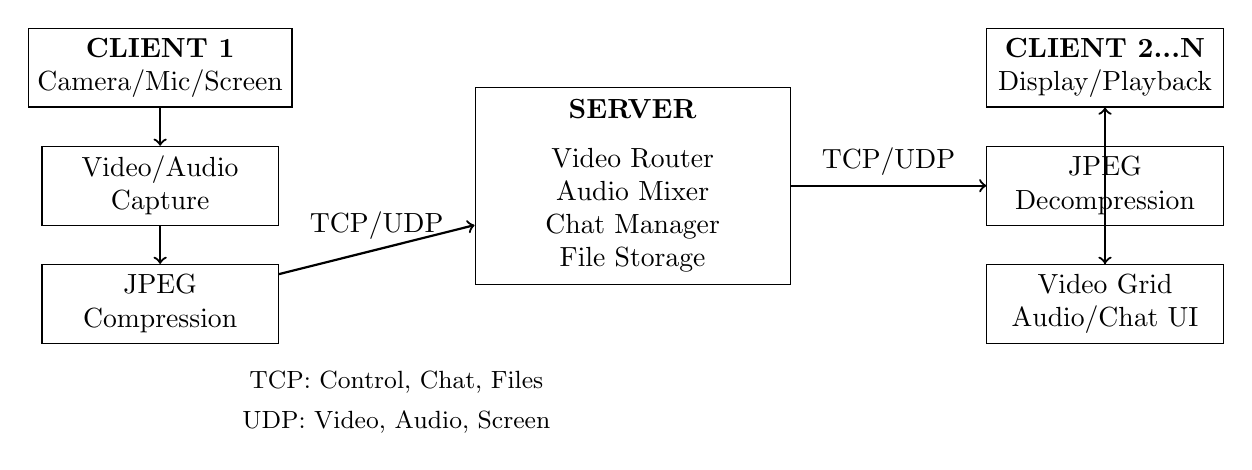
\begin{tikzpicture}[
        box/.style={rectangle, draw, minimum width=3cm, minimum height=1cm, align=center},
        arrow/.style={->, thick}
    ]
        % Client 1
        \node[box] (client1) at (0,4) {\textbf{CLIENT 1}\\ Camera/Mic/Screen};
        \node[box] (client1-cap) at (0,2.5) {Video/Audio\\Capture};
        \node[box] (client1-enc) at (0,1) {JPEG\\Compression};
        
        % Server
        \node[box, minimum width=4cm, minimum height=2.5cm] (server) at (6,2.5) {
            \textbf{SERVER}\\[0.2cm]
            Video Router\\
            Audio Mixer\\
            Chat Manager\\
            File Storage
        };
        
        % Client 2-N
        \node[box] (clientN) at (12,4) {\textbf{CLIENT 2...N}\\ Display/Playback};
        \node[box] (clientN-dec) at (12,2.5) {JPEG\\Decompression};
        \node[box] (clientN-ui) at (12,1) {Video Grid\\Audio/Chat UI};
        
        % Arrows
        \draw[arrow] (client1) -- (client1-cap);
        \draw[arrow] (client1-cap) -- (client1-enc);
        \draw[arrow] (client1-enc) -- node[above] {TCP/UDP} (server);
        \draw[arrow] (server) -- node[above] {TCP/UDP} (clientN-dec);
        \draw[arrow] (clientN-dec) -- (clientN-ui);
        \draw[arrow] (clientN-ui) -- (clientN);
        
        % Protocols
        \node[draw=none, font=\small] at (3,0) {TCP: Control, Chat, Files};
        \node[draw=none, font=\small] at (3,-0.5) {UDP: Video, Audio, Screen};
    \end{tikzpicture}
    \caption{High-Level System Architecture}
    \label{fig:system-arch}
\end{figure}

\begin{figure}[H]
    \centering
    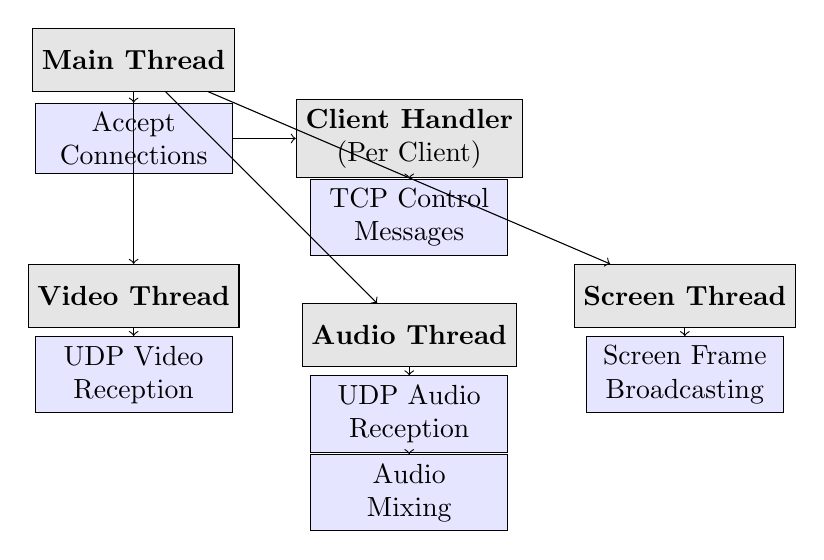
\begin{tikzpicture}[
        component/.style={rectangle, draw, minimum width=2.5cm, minimum height=0.8cm, align=center, fill=gray!20},
        thread/.style={rectangle, draw, minimum width=2.5cm, minimum height=0.6cm, align=center, fill=blue!10}
    ]
        \node[component] (main) at (0,0) {\textbf{Main Thread}};
        \node[thread] (conn) at (0,-1) {Accept\\Connections};
        
        \node[component] (client) at (3.5,-1) {\textbf{Client Handler}\\(Per Client)};
        \node[thread] (tcp) at (3.5,-2) {TCP Control\\Messages};
        
        \node[component] (video) at (0,-3) {\textbf{Video Thread}};
        \node[thread] (vid-rx) at (0,-4) {UDP Video\\Reception};
        
        \node[component] (audio) at (3.5,-3.5) {\textbf{Audio Thread}};
        \node[thread] (aud-rx) at (3.5,-4.5) {UDP Audio\\Reception};
        \node[thread] (aud-mix) at (3.5,-5.5) {Audio\\Mixing};
        
        \node[component] (screen) at (7,-3) {\textbf{Screen Thread}};
        \node[thread] (scr-rx) at (7,-4) {Screen Frame\\Broadcasting};
        
        \draw[->] (main) -- (conn);
        \draw[->] (conn) -- (client);
        \draw[->] (client) -- (tcp);
        \draw[->] (main) -- (video);
        \draw[->] (video) -- (vid-rx);
        \draw[->] (main) -- (audio);
        \draw[->] (audio) -- (aud-rx);
        \draw[->] (aud-rx) -- (aud-mix);
        \draw[->] (main) -- (screen);
        \draw[->] (screen) -- (scr-rx);
    \end{tikzpicture}
    \caption{Server Threading Architecture}
    \label{fig:server-threads}
\end{figure}

% ============================================================================
% CHAPTER 3: PROTOCOL DESIGN
% ============================================================================
\chapter{Protocol Design}

\section{Message Format}

\subsection{Text-Based Messages (TCP)}
Format: \texttt{COMMAND:field1:field2:...}

Examples:
\begin{itemize}[itemsep=3pt]
    \item \texttt{CONNECT:username} - User connection request
    \item \texttt{CHAT:sender:message} - Group chat message
    \item \texttt{PRIVATE\_CHAT:sender:recipient:message} - Private message
    \item \texttt{FILE\_UPLOAD:filename:size:chunk\_data} - File upload
\end{itemize}

\subsection{Binary Messages (UDP)}
Format: \texttt{COMMAND + 4-byte length + binary data}

\section{Protocol Categories}

\subsection{Connection Protocol}
\begin{table}[H]
\centering
\caption{Connection Messages}
\begin{tabular}{lll}
\toprule
\textbf{Message} & \textbf{Direction} & \textbf{Purpose} \\
\midrule
\rowcolor{gray!20}
CONNECT:username & C→S & Join conference \\
CONNECT\_SUCCESS & S→C & Confirm connection \\
\rowcolor{gray!20}
DISCONNECT & C→S/S→C & Leave conference \\
USER\_LIST:user1,user2,... & S→C & Update participant list \\
\bottomrule
\end{tabular}
\end{table}

\subsection{Media Control Protocol}
\begin{table}[H]
\centering
\caption{Media Control Messages}
\begin{tabular}{lll}
\toprule
\textbf{Message} & \textbf{Direction} & \textbf{Purpose} \\
\midrule
\rowcolor{gray!20}
START\_VIDEO & C→S & Begin video streaming \\
STOP\_VIDEO & C→S & End video streaming \\
\rowcolor{gray!20}
START\_AUDIO & C→S & Begin audio streaming \\
STOP\_AUDIO & C→S & End audio streaming \\
\rowcolor{gray!20}
VIDEO\_FRAME:user:data & UDP & Video frame transmission \\
AUDIO\_CHUNK:user:data & UDP & Audio chunk transmission \\
\bottomrule
\end{tabular}
\end{table}

\subsection{Chat Protocol}
\begin{table}[H]
\centering
\caption{Chat Messages}
\begin{tabular}{lll}
\toprule
\textbf{Message} & \textbf{Direction} & \textbf{Purpose} \\
\midrule
\rowcolor{gray!20}
CHAT:sender:message & C→S→C & Group message \\
PRIVATE\_CHAT:sender:recipient:msg & C→S→C & Private message \\
\rowcolor{gray!20}
CHAT\_HISTORY:messages & S→C & Load message history \\
\bottomrule
\end{tabular}
\end{table}

\subsection{Screen Sharing Protocol}
\begin{table}[H]
\centering
\caption{Screen Sharing Messages}
\begin{tabular}{lll}
\toprule
\textbf{Message} & \textbf{Direction} & \textbf{Purpose} \\
\midrule
\rowcolor{gray!20}
REQUEST\_PRESENTER & C→S & Request presenter role \\
GRANT\_PRESENTER:user & S→C & Approve presenter \\
\rowcolor{gray!20}
DENY\_PRESENTER & S→C & Reject presenter request \\
STOP\_SCREEN\_SHARE & C→S/S→C & End screen sharing \\
\rowcolor{gray!20}
SCREEN\_FRAME:data & UDP & Screen frame data \\
\bottomrule
\end{tabular}
\end{table}

\section{Media Encoding}

\subsection{Video Processing}
\begin{itemize}[itemsep=5pt]
    \item \textbf{Resolution:} 640x480 (VGA), downscaled from camera input
    \item \textbf{Format:} BGR to RGB conversion via OpenCV
    \item \textbf{Compression:} JPEG encoding (quality=80)
    \item \textbf{Frame Rate:} 15 FPS (adaptive based on network)
    \item \textbf{Transport:} UDP with 16KB chunks
\end{itemize}

\subsection{Audio Processing}
\begin{itemize}[itemsep=5pt]
    \item \textbf{Sample Rate:} 44100 Hz
    \item \textbf{Channels:} Mono (1 channel)
    \item \textbf{Format:} 16-bit PCM (paInt16)
    \item \textbf{Chunk Size:} 1024 frames
    \item \textbf{Mixing:} Server-side averaging with volume normalization
    \item \textbf{Jitter Buffer:} 100ms buffer for smooth playback
\end{itemize}

\subsection{Screen Sharing}
\begin{itemize}[itemsep=5pt]
    \item \textbf{Capture:} MSS library for full-screen capture
    \item \textbf{Compression:} JPEG (quality=60) for bandwidth efficiency
    \item \textbf{Frame Rate:} 5-10 FPS (lower for bandwidth conservation)
    \item \textbf{Access Control:} Single presenter at a time
\end{itemize}

% ============================================================================
% CHAPTER 4: IMPLEMENTATION DETAILS
% ============================================================================
\chapter{Implementation Details}

\section{Core Implementation Functions}

\subsection{Server Implementation}

\subsubsection{Connection Management}
\begin{itemize}[itemsep=3pt]
    \item \texttt{start\_server()}: Initialize server sockets and threads
    \item \texttt{accept\_connections()}: Handle new client connections
    \item \texttt{handle\_client(socket)}: Process client control messages
    \item \texttt{broadcast\_user\_list()}: Send updated participant list
    \item \texttt{handle\_disconnect(username)}: Clean up client resources
\end{itemize}

\subsubsection{Video Handling}
\begin{itemize}[itemsep=3pt]
    \item \texttt{receive\_video\_frames()}: UDP video reception loop
    \item \texttt{broadcast\_video\_frame(user, frame)}: Distribute video to clients
    \item \texttt{decode\_video\_frame(data)}: JPEG decompression
    \item \texttt{update\_video\_grid()}: Manage grid layout on clients
\end{itemize}

\subsubsection{Audio Handling}
\begin{itemize}[itemsep=3pt]
    \item \texttt{receive\_audio\_chunks()}: UDP audio reception
    \item \texttt{mix\_audio\_streams()}: Combine multiple audio sources
    \item \texttt{normalize\_audio(data)}: Volume level adjustment
    \item \texttt{broadcast\_mixed\_audio()}: Send mixed audio to clients
\end{itemize}

\subsubsection{Chat Management}
\begin{itemize}[itemsep=3pt]
    \item \texttt{handle\_group\_message(sender, msg)}: Broadcast group chat
    \item \texttt{handle\_private\_message(sender, recipient, msg)}: Route PM
    \item \texttt{send\_chat\_history(client)}: Load message history
    \item \texttt{store\_message(message)}: Persist chat messages
\end{itemize}

\subsubsection{File Transfer}
\begin{itemize}[itemsep=3pt]
    \item \texttt{handle\_file\_upload(filename, size, chunks)}: Receive file
    \item \texttt{handle\_file\_download(filename)}: Send file to client
    \item \texttt{broadcast\_file\_available(metadata)}: Notify clients
    \item \texttt{track\_upload\_progress(bytes)}: Update progress
\end{itemize}

\subsubsection{Screen Sharing}
\begin{itemize}[itemsep=3pt]
    \item \texttt{grant\_presenter\_role(username)}: Assign presenter
    \item \texttt{revoke\_presenter\_role()}: Remove presenter
    \item \texttt{broadcast\_screen\_frame(frame)}: Distribute screen
    \item \texttt{handle\_stop\_screen\_share()}: End presentation
\end{itemize}

\subsection{Client Implementation}

\subsubsection{Connection}
\begin{itemize}[itemsep=3pt]
    \item \texttt{connect\_to\_server(host, port, username)}: Establish connection
    \item \texttt{receive\_messages()}: TCP message reception thread
    \item \texttt{send\_heartbeat()}: Keep-alive mechanism
    \item \texttt{handle\_disconnect()}: Clean shutdown
\end{itemize}

\subsubsection{Video Capture}
\begin{itemize}[itemsep=3pt]
    \item \texttt{initialize\_camera()}: Open cv2.VideoCapture
    \item \texttt{capture\_video\_thread()}: Frame capture loop
    \item \texttt{encode\_frame(frame)}: JPEG compression
    \item \texttt{send\_video\_frame(data)}: UDP transmission
    \item \texttt{toggle\_video()}: Start/stop video
\end{itemize}

\subsubsection{Video Display}
\begin{itemize}[itemsep=3pt]
    \item \texttt{receive\_video\_frames()}: UDP reception
    \item \texttt{display\_video\_frame(user, frame)}: Show in grid
    \item \texttt{create\_video\_grid\_layout()}: Dynamic grid sizing
    \item \texttt{update\_video\_label(user, pixmap)}: Qt UI update
\end{itemize}

\subsubsection{Audio Capture}
\begin{itemize}[itemsep=3pt]
    \item \texttt{initialize\_audio()}: PyAudio stream setup
    \item \texttt{capture\_audio\_thread()}: Recording loop
    \item \texttt{send\_audio\_chunk(data)}: UDP transmission
    \item \texttt{toggle\_audio()}: Mute/unmute
\end{itemize}

\subsubsection{Audio Playback}
\begin{itemize}[itemsep=3pt]
    \item \texttt{receive\_audio\_chunks()}: UDP reception
    \item \texttt{fill\_jitter\_buffer(chunk)}: Buffer management
    \item \texttt{playback\_audio\_thread()}: Playback loop
    \item \texttt{adjust\_playback\_rate()}: Sync correction
\end{itemize}

\subsubsection{Screen Sharing}
\begin{itemize}[itemsep=3pt]
    \item \texttt{request\_presenter\_role()}: Send presenter request
    \item \texttt{start\_screen\_capture()}: MSS capture initialization
    \item \texttt{capture\_screen\_thread()}: Screen capture loop
    \item \texttt{display\_screen\_share(frame)}: Show presenter screen
    \item \texttt{stop\_screen\_share()}: End presentation
\end{itemize}

\subsubsection{Chat}
\begin{itemize}[itemsep=3pt]
    \item \texttt{send\_group\_message(text)}: Broadcast message
    \item \texttt{send\_private\_message(recipient, text)}: Send PM
    \item \texttt{display\_chat\_message(sender, msg, private)}: Show in UI
    \item \texttt{load\_chat\_history()}: Retrieve history
    \item \texttt{show\_notification(message)}: Chat alerts
\end{itemize}

\subsubsection{File Sharing}
\begin{itemize}[itemsep=3pt]
    \item \texttt{select\_file()}: File picker dialog
    \item \texttt{upload\_file(filepath)}: Chunked upload
    \item \texttt{download\_file(file\_id)}: Request download
    \item \texttt{update\_file\_list(files)}: Refresh available files
    \item \texttt{show\_upload\_progress(percent)}: Progress dialog
\end{itemize}

\subsubsection{UI Components}
\begin{itemize}[itemsep=3pt]
    \item \texttt{create\_main\_window()}: Application window setup
    \item \texttt{create\_control\_bar()}: Media control buttons
    \item \texttt{create\_side\_panel()}: Chat/People/Files tabs
    \item \texttt{create\_video\_area()}: Video grid container
    \item \texttt{show\_connection\_dialog()}: Server connection UI
    \item \texttt{apply\_dark\_theme()}: Dark mode styling
\end{itemize}

\section{Error Handling}

\begin{itemize}[itemsep=5pt]
    \item \textbf{Connection Errors:} Timeout handling, reconnection attempts
    \item \textbf{Camera Errors:} Graceful fallback if camera unavailable
    \item \textbf{Audio Errors:} Device detection and error messages
    \item \textbf{Network Errors:} Packet loss handling, buffer underrun recovery
    \item \textbf{File Transfer Errors:} Corrupted chunk detection, retry mechanism
\end{itemize}

% ============================================================================
% CHAPTER 5: INSTALLATION AND USAGE
% ============================================================================
\chapter{Installation and Usage}

\section{System Requirements}

\subsection{Hardware}
\begin{itemize}[itemsep=3pt]
    \item \textbf{Processor:} Dual-core 2.0 GHz or better
    \item \textbf{RAM:} 4GB minimum (8GB recommended)
    \item \textbf{Network:} 100 Mbps LAN or better
    \item \textbf{Webcam:} 720p or higher
    \item \textbf{Microphone:} Any USB or built-in microphone
\end{itemize}

\subsection{Software}
\begin{itemize}[itemsep=3pt]
    \item Python 3.8 or higher
    \item Windows 10/11, Linux, or macOS
    \item Required packages: PyQt6, OpenCV, PyAudio, NumPy, MSS
\end{itemize}

\section{Installation Steps}

\subsection{Install Python Dependencies}
\begin{verbatim}
pip install -r requirements.txt
\end{verbatim}


\subsection{Run Server}
\begin{verbatim}
python src/server/server.py
# Default port: 12345 (TCP), 12346 (UDP video), 12347 (UDP audio)
\end{verbatim}

\subsection{Run Client}
\begin{verbatim}
python src/client/client.py
# Enter server IP and username in connection dialog
\end{verbatim}

Alternatively, you could build the client and server and run the executables (i.e., the ones we have submitted)

\section{Quick Start Guide}

\subsection{Connecting}
\begin{enumerate}[itemsep=3pt]
    \item Launch client application
    \item Enter server IP address (e.g., 192.168.1.100)
    \item Choose unique username
    \item Click Connect
\end{enumerate}

\subsection{Video Conferencing}
\begin{enumerate}[itemsep=3pt]
    \item Click "Start Video" to enable camera
    \item Video appears in grid with other participants
    \item Click "Stop Video" to disable
\end{enumerate}

\subsection{Audio}
\begin{enumerate}[itemsep=3pt]
    \item Click "Unmute" to enable microphone
    \item Audio automatically mixed on server
    \item Use headphones to prevent echo
\end{enumerate}

\subsection{Screen Sharing}
\begin{enumerate}[itemsep=3pt]
    \item Click "Share Screen"
    \item Wait for presenter approval (first-come-first-served)
    \item Screen appears to all participants
    \item Click "Stop Sharing" to end
\end{enumerate}

\subsection{Chat}
\begin{enumerate}[itemsep=3pt]
    \item Select "Chat" tab in side panel
    \item Type message and press Enter for group chat
    \item Click "PM" button for private messages
\end{enumerate}

\subsection{File Sharing}
\begin{enumerate}[itemsep=3pt]
    \item Select "Files" tab
    \item Click "Upload File" to share
    \item Click "Download" next to file to receive
\end{enumerate}

% ============================================================================
% CHAPTER 6: APPLICATION SCREENSHOTS
% ============================================================================
\chapter{Application Screenshots}

\section{Main Application Interface}

\begin{figure}[H]
    \centering
    \includegraphics[width=0.9\textwidth]{../screenshots/MainApplicationWindow.jpg}
    \caption{Main Application Interface}
    \label{fig:main-interface}
\end{figure}

\section{Connection Dialog}

\begin{figure}[H]
    \centering
    \includegraphics[width=0.6\textwidth]{../screenshots/JoiningWindow.jpg}
    \caption{Joining Window (Server IP and Username Entry)}
    \label{fig:connection-dialog}
\end{figure}

\section{Video Conferencing}

\begin{figure}[H]
    \centering
    \includegraphics[width=0.9\textwidth]{../screenshots/TiledLayout.jpg}
    \caption{Video Conference with Multiple Participants in Tiled Layout}
    \label{fig:video-conference}
\end{figure}

\section{Screen Sharing}

\begin{figure}[H]
    \centering
    \includegraphics[width=0.9\textwidth]{../screenshots/TiledLayoutWithScreenShare.jpg}
    \caption{Screen Sharing in Tiled Layout View}
    \label{fig:screen-sharing-tiled}
\end{figure}

\begin{figure}[H]
    \centering
    \includegraphics[width=0.9\textwidth]{../screenshots/SpotlightWithScreenShare.jpg}
    \caption{Screen Sharing in Spotlight Layout View}
    \label{fig:screen-sharing-spotlight}
\end{figure}

\section{Chat Interface}

\begin{figure}[H]
    \centering
    \includegraphics[width=0.7\textwidth]{../screenshots/ChatWindow.jpg}
    \caption{Chat Interface}
    \label{fig:chat-interface}
\end{figure}

\section{Participants Panel}

\begin{figure}[H]
    \centering
    \includegraphics[width=0.6\textwidth]{../screenshots/Participants.jpg}
    \caption{Participants Panel}
    \label{fig:participants-panel}
\end{figure}

\section{File Sharing Panel}

\begin{figure}[H]
    \centering
    \includegraphics[width=0.7\textwidth]{../screenshots/FilePicker.jpg}
    \caption{File Sharing Panel with File Picker}
    \label{fig:file-sharing}
\end{figure}

\begin{figure}[H]
    \centering
    \includegraphics[width=0.6\textwidth]{../screenshots/DeleteOwnUploadWarning.jpg}
    \caption{Delete File Warning Dialog}
    \label{fig:delete-file-warning}
\end{figure}

\section{Settings Panel}

\begin{figure}[H]
    \centering
    \includegraphics[width=0.8\textwidth]{../screenshots/Settings.jpg}
    \caption{Settings Panel}
    \label{fig:settings-panel}
\end{figure}

\section{Notifications}

\begin{figure}[H]
    \centering
    \includegraphics[width=0.8\textwidth]{../screenshots/JoinNotif.jpg}
    \caption{User Join Notification}
    \label{fig:join-notification}
\end{figure}

\begin{figure}[H]
    \centering
    \includegraphics[width=0.8\textwidth]{../screenshots/LeaveNotif.jpg}
    \caption{User Leave Notification}
    \label{fig:leave-notification}
\end{figure}

\begin{figure}[H]
    \centering
    \includegraphics[width=0.8\textwidth]{../screenshots/ChatNotif.jpg}
    \caption{Chat Message Notification}
    \label{fig:chat-notification}
\end{figure}

\section{Private Chat}

\begin{figure}[H]
    \centering
    \includegraphics[width=0.7\textwidth]{../screenshots/PrivateChatExample.jpg}
    \caption{Private Chat to Individual Users}
    \label{fig:private-chat}
\end{figure}

\section{Video Layout Modes}

\begin{figure}[H]
    \centering
    \includegraphics[width=0.9\textwidth]{../screenshots/TiledLayout.jpg}
    \caption{Tiled Layout View}
    \label{fig:tiled-layout}
\end{figure}

\begin{figure}[H]
    \centering
    \includegraphics[width=0.9\textwidth]{../screenshots/SpotlightWithScreenShare.jpg}
    \caption{Spotlight Layout View}
    \label{fig:spotlight-layout}
\end{figure}

\begin{figure}[H]
    \centering
    \includegraphics[width=0.6\textwidth]{../screenshots/LayoutOptions.jpg}
    \caption{Layout Selection Options}
    \label{fig:layout-options}
\end{figure}

\section{Connection Dialog}

\begin{figure}[H]
    \centering
    \includegraphics[width=0.6\textwidth]{../screenshots/JoiningWindow.jpg}
    \caption{Joining Window (Server IP and Username Entry)}
    \label{fig:joining-window}
\end{figure}

\section{Screen Share Warning}

\begin{figure}[H]
    \centering
    \includegraphics[width=0.7\textwidth]{../screenshots/ScreenShareUnavailable.jpg}
    \caption{Screen Share Conflict Warning Dialog}
    \label{fig:screenshare-warning}
\end{figure}

% ============================================================================
% CHAPTER 7: CONCLUSION AND FUTURE WORK
% ============================================================================
\chapter{Conclusion and Future Work}

\section{Conclusion}

This project successfully demonstrates a comprehensive LAN-based video conferencing solution operating without internet connectivity. The implementation achieves all primary objectives:

\begin{itemize}[itemsep=5pt]
    \item Multi-user video conferencing with up to 10 participants
    \item Server-side audio mixing with acceptable latency (<150ms)
    \item Presenter-controlled screen sharing
    \item Group and private messaging with history
    \item File sharing with progress tracking
    \item Robust error handling and graceful disconnection
\end{itemize}

The system provides a practical solution for secure, local communication in environments where internet access is limited or restricted, such as educational institutions, secure facilities, and emergency response scenarios.

Key achievements include:
\begin{itemize}[itemsep=5pt]
    \item Custom protocol design for efficient media streaming
    \item Scalable multi-threaded server architecture
    \item Responsive PyQt6-based user interface
    \item Real-time performance with minimal latency
    \item Cross-platform compatibility
\end{itemize}

\section{Future Enhancements}

\subsection{Security Improvements}
\begin{itemize}[itemsep=3pt]
    \item Implement TLS/SSL for encrypted connections
    \item Add user authentication with passwords
    \item End-to-end encryption for private messages
    \item Role-based access control (admin, moderator, participant)
\end{itemize}

\subsection{Performance Optimizations}
\begin{itemize}[itemsep=3pt]
    \item Adaptive bitrate for video based on network conditions
    \item H.264 hardware encoding for better compression
    \item Multicast for video distribution (reduce bandwidth)
    \item WebRTC integration for peer-to-peer capabilities
\end{itemize}

\subsection{Feature Additions}
\begin{itemize}[itemsep=3pt]
    \item Virtual backgrounds and filters for video
    \item Recording and playback of conferences
    \item Whiteboard/collaborative drawing tool
    \item Polls and Q\&A features
    \item Breakout rooms for smaller groups
    \item Mobile client support (Android/iOS)
\end{itemize}

\subsection{Quality Improvements}
\begin{itemize}[itemsep=3pt]
    \item Echo cancellation algorithms
    \item Noise suppression for audio
    \item Automatic gain control
    \item Better jitter buffer management
    \item Packet loss concealment
\end{itemize}

\subsection{Scalability}
\begin{itemize}[itemsep=3pt]
    \item Distributed server architecture for load balancing
    \item Support for 50+ participants
    \item Database integration for persistent storage
    \item Web-based client (browser access)
\end{itemize}

\section{Lessons Learned}

\begin{itemize}[itemsep=5pt]
    \item \textbf{Threading Complexity:} Managing multiple concurrent threads requires careful synchronization and deadlock prevention
    \item \textbf{Network Variability:} Real-world networks have unpredictable latency and packet loss requiring robust handling
    \item \textbf{UI Responsiveness:} Separating network I/O from UI thread is critical for smooth user experience
    \item \textbf{Resource Management:} Proper cleanup of threads, sockets, and media devices prevents resource leaks
    \item \textbf{Protocol Design:} Clear, extensible protocol design simplifies debugging and future enhancements
\end{itemize}

\section{Final Remarks}

This project demonstrates that effective video conferencing solutions can be built for LAN environments using standard Python libraries and socket programming. The system provides a foundation for further development and customization based on specific organizational needs.

The implementation showcases practical applications of computer networks concepts including:
\begin{itemize}[itemsep=3pt]
    \item Client-server architecture
    \item TCP/UDP protocol usage
    \item Multimedia streaming
    \item Concurrent programming
    \item Real-time system design
\end{itemize}

\end{document}
